\documentclass[11pt, a4paper]{article} % Formato del documento
\usepackage[spanish, english]{babel} % Idiomas
\usepackage{amsfonts, amsmath, amssymb} % Símbolos matemáticos
\usepackage{hyperref} % Referencias
\usepackage{graphicx} % Insertar imágenes
\usepackage{float} % Para agregar imagen en el lugar
\usepackage{tikz} % Insertar gráficos
\usepackage{siunitx} % Insertar ángulos
\usepackage{apacite}  % Citaciones en formato apa
\usepackage[a4paper, top=30mm, bottom=20mm, left=30mm, right=30mm]{geometry} % Márgenes y tamaño del documento
\usepackage{caption} % Para subfiguras
\usepackage{subcaption}
\usepackage{setspace} % Interlineado
\usepackage{fancyhdr}

% Reference settings
\hypersetup{
    colorlinks=true,
    linkcolor=blue,
    filecolor=magenta,      
    urlcolor=cyan,
    citecolor=cyan,
    pdftitle={TP1 - cuadránte astronómico - Cavalieri y Chen},
    pdfpagemode=FullScreen,
}

% Header
\fancyhead[LH]{TP1 Astronomía cuadrantes}
\fancyhead[RH]{TP1 Astronomía cuadrantes}


% Información del documento
\title{Trabajo Práctico Nº1 \\ Cuadrante astronómico}
\author{Lola Cavalieri e Ian Chen}
\date{11 de junio de 2024}


%---------------------------
\begin{document}
\selectlanguage{spanish}
\maketitle
\onehalfspacing
\vspace{1cm}
% RESUMEN Y ABSTRACT
\begin{abstract}
  En este informe se desarrolla un análisis de la latitud del lugar de observación, mediante mediciones y observaciones de las alturas de estrellas como Acrux y Mimosa con el uso de un cuadrante hecho a mano por nosotros mismos como herramienta principal, y relacionando conceptos de altura, declinación, latitud y meridiano del lugar, con el fin de hallar de forma analítica la latitud del lugar de observación ($\overline{\varphi} = -\ang{34} \,22\text{'}\, 52\text{''} \pm 3$). La medición se realizó desde el observatorio de astronomía del Colegio Nacional de Buenos Aires el día 16 de mayo de 2024, entre las horas 21:56 y 22:19 (GMT-3). Se realizaron tablas de las mediciones y gráficos con los valores obtenidos tanto por nuestro grupo como por todos grupos del curso, para conseguir un valor final más exacto. Al final se obtuvieron los datos esperados desde un principio, por lo que se considera que el proceso experimental obtuvo un buen resultado.
\end{abstract}

\selectlanguage{english}
\begin{abstract}
This report analyzes the altitude of various stars using a homemade quadrant as the main tool to determine the observer's latitude and to relate the concepts of altitude, declination, latitude, and the local meridian, in order to analytically determine the latitude of the observation site ($\overline{\varphi} = -\ang{34} \,22\text{'}\, 52\text{''} \pm 3$). The experiment was performed over Acrux and Mimosa, from the observatory of the Colegio Nacional de Buenos Aires, on May 16th of 2024, between 21:56 and 22:19 (GMT-3).  To achieve this, tables and graphs were created with the values collected by our group as well as by all the groups in the course, in order to reach a more accurate final value. In the end, the expected data were obtained, indicating that the experimental process yielded good results.
\end{abstract}

\selectlanguage{spanish}
\newpage


%-------------------------------
\section{Introducción}
En el presente trabajo práctico procederemos a calcular la latitud del lugar por medio de la medición y observación de astros. 
Las mediciones se realizaron en la terraza del observatorio de astronomía del Colegio Nacional de Buenos Aires el día 16 de mayo de 2024, entre las horas 21:56 y 22:19 (GMT-3). 
Es presentado en el contexto de la asignatura de “Astronomía”, abordando temas como el estudio de coordenadas astronómicas (acimutales y ecuatoriales) y relacionando conceptos básicos como altura, declinación, latitud, meridiano del lugar, cenit, nadir, entre otros.
Estos temas fueron dados durante la cursada, y el Trabajo Práctico propone como objetivo poder aplicar los conocimientos aprendidos, así como llevar a cabo un procedimiento experimental científico.


%-------------------------------
\section{Desarrollo experimental}
Para ubicarnos geográficamente utilizamos en primer momento la aplicación “Google Maps”, en su función de brújula, por sobre nuestros conocimientos previos tomando en cuenta que el observatorio se encuentra en la zona de microcentro, y el Río de la Plata (visible desde el punto de observación) se encuentra al este. Además contamos con la información proporcionada por la docente a cargo de la posición aproximada del Polo Sur Celeste (PSC) en el cielo desde el lugar de observación. Luego se procedió a ubicar el “Meridiano del Lugar”, el cual es el meridiano celeste que contiene tanto los polos celestes como el Cenit y Nadir. Este es importante para el análisis de este trabajo ya que las estrellas elegidas para la observación (Acrux y Becrux) debían estar cerca del mismo, puesto que de esta forma se podría relacionar los dos tipos de sistemas (acimutal y ecuatorial) en un mismo plano, y generar ecuaciones que involucren declinación y altura de las estrellas. 

La deducción de las fórmulas que relaciona la latitud del lugar con la declinación de una estrella y su altura en la culminación superior daban seis casos posibles (3 por cada hemisferio): que la estrella esté entre el horizonte y el Ecuador Celeste, entre el Ecuador celeste y el Polo celeste, y entre el Polo celeste y el Horizonte. Estas 6 ecuaciones se pueden hallar en el apéndice del documento. 
Para nuestro caso utilizamos la ecuación del caso en el que la estrella se encuentra entre Ecuador Celeste y Polo Sur Celeste como se observa en Figura 1:

% -----------IMAGEN ECUACIONES------------
\selectlanguage{english}
\begin{figure}[H]
    \centering
    \begin{tikzpicture}[scale=1]
    % Circunferencia
    \draw[black, thick] (0,0) circle (3);
    
    % Rectas / Líneas
    \draw[black, thin] (-3, 0) -- (3, 0) node[anchor=west]{Horizonte};
    \draw[black, thin] (-2.48, -1.68) -- (2.48, 1.68) node[anchor=south west]{Polo Sur Celeste};
    \draw[black, thin]  (1.68, -2.48) -- (-1.68, 2.48)  node[anchor=south east]{Ecuador Celeste};
    % Recta roja del punto
    \draw[red!70, dashed] (0,0) -- (0,3);

    % Arcos
    % Declinación
    \draw[->, cyan!50, ultra thick] (-1.68, 2.55) arc (124:95:3.1) node[midway, above]{$\delta$};
    % Altura
    \draw[blue!40, ultra thick, ->] (3.1, 0) arc (0:85:3.1) node[anchor=south west]{$h$};
    % Ángulo en rosa
    \fill[fill=red!20, opacity=0.5] (0,0) -- (2.48, 1.68) arc (34:90:3);
    % LATITUD (NO CAMBIAR)
    \draw[black, thick, ->] (1, 0) arc (0:34:1) node[midway, right]{$\varphi$};
    
    % Cuadrados
    \draw[black, thin, rotate around={34:(0,0)}] (0,0) rectangle (0.3, 0.35);

    % Puntos
    % Centro
    \filldraw[fill=black!50, draw=black!50] (0,0) circle (0.1);
    % Estrella
    \filldraw[fill=yellow, draw=yellow] (0,3) circle (0.1); % Estrella en angulo 90º
\end{tikzpicture}
    \caption{Estrella entre Ecuador Celeste y Polo Sur Celeste}
    \label{fig:case-1}
\end{figure}
\selectlanguage{spanish}

%---------------------------------
Antes que nada se debe saber que el ángulo comprendido entre ecuador celeste y polo sur celeste es por definición $\ang{90}$.

Para establecer una relación, podemos observar que $\ang{90}-|\delta|$ es igual al ángulo en rosa. Y esa misma área es igual a la altura menos la latitud $|h|-|\varphi|$, por lo que $\ang{90}-\delta = h-\varphi$. Despejando todo finalmente se obtiene que $\varphi=\ang{90}+\delta - h$, que es la ecuación utilizada en el trabajo para hallar la latitud. 

Se estableció un valor de $\ang{3}$ para las mediciones de altura ($\varepsilon h = \ang{3}$), considerando la incerteza del instrumento, el criterio del observador y las condiciones del viento. Luego se obtuvo un valor promedio de latitud de $\overline{\varphi} = -\ang{34} \,22\text{'}\, 52\text{''}$, al cual se le asignó una incerteza de $\ang{3}$ ($\varepsilon \overline{\varphi}=\ang{3}$). Esta se determinó  mediante la propagación de incertezas de la altura (véase el apéndice).

Con respecto a la estimación aproximada del meridiano del lugar durante las mediciones, la estrella tiene sus puntos máximos de variación en su altura en los puntos este y oeste, y su movimiento aparente es mucho más veloz. Por el contrario, cuando se encuentra en su culminación superior, que es cuando se encuentra exactamente cruzando el meridiano del lugar, la variación de su altura es mínima y su movimiento aparente mucho más lento, por lo que los errores en el  posicionamiento exacto de la dirección Norte–Sur y de la estrella son despreciables a la hora de tomar mediciones.

Por último con las 40 mediciones tomadas (20 por cada estrella) se confeccionó una tabla, y una vez completada, se procedió a realizar un histograma con la distribución estadística de los valores de la latitud obtenidos por todos los grupos del curso. Por otra parte, también se confeccionó un gráfico para un análisis más detallado. Tanto el histograma como el gráfico se realizaron con Python.


%---------------------------------
\section{Resultado y análisis}
\subsection{Tabla de mediciones}
% Análisis de Tabla de mediciones
\begin{figure}[H]
    \centering
    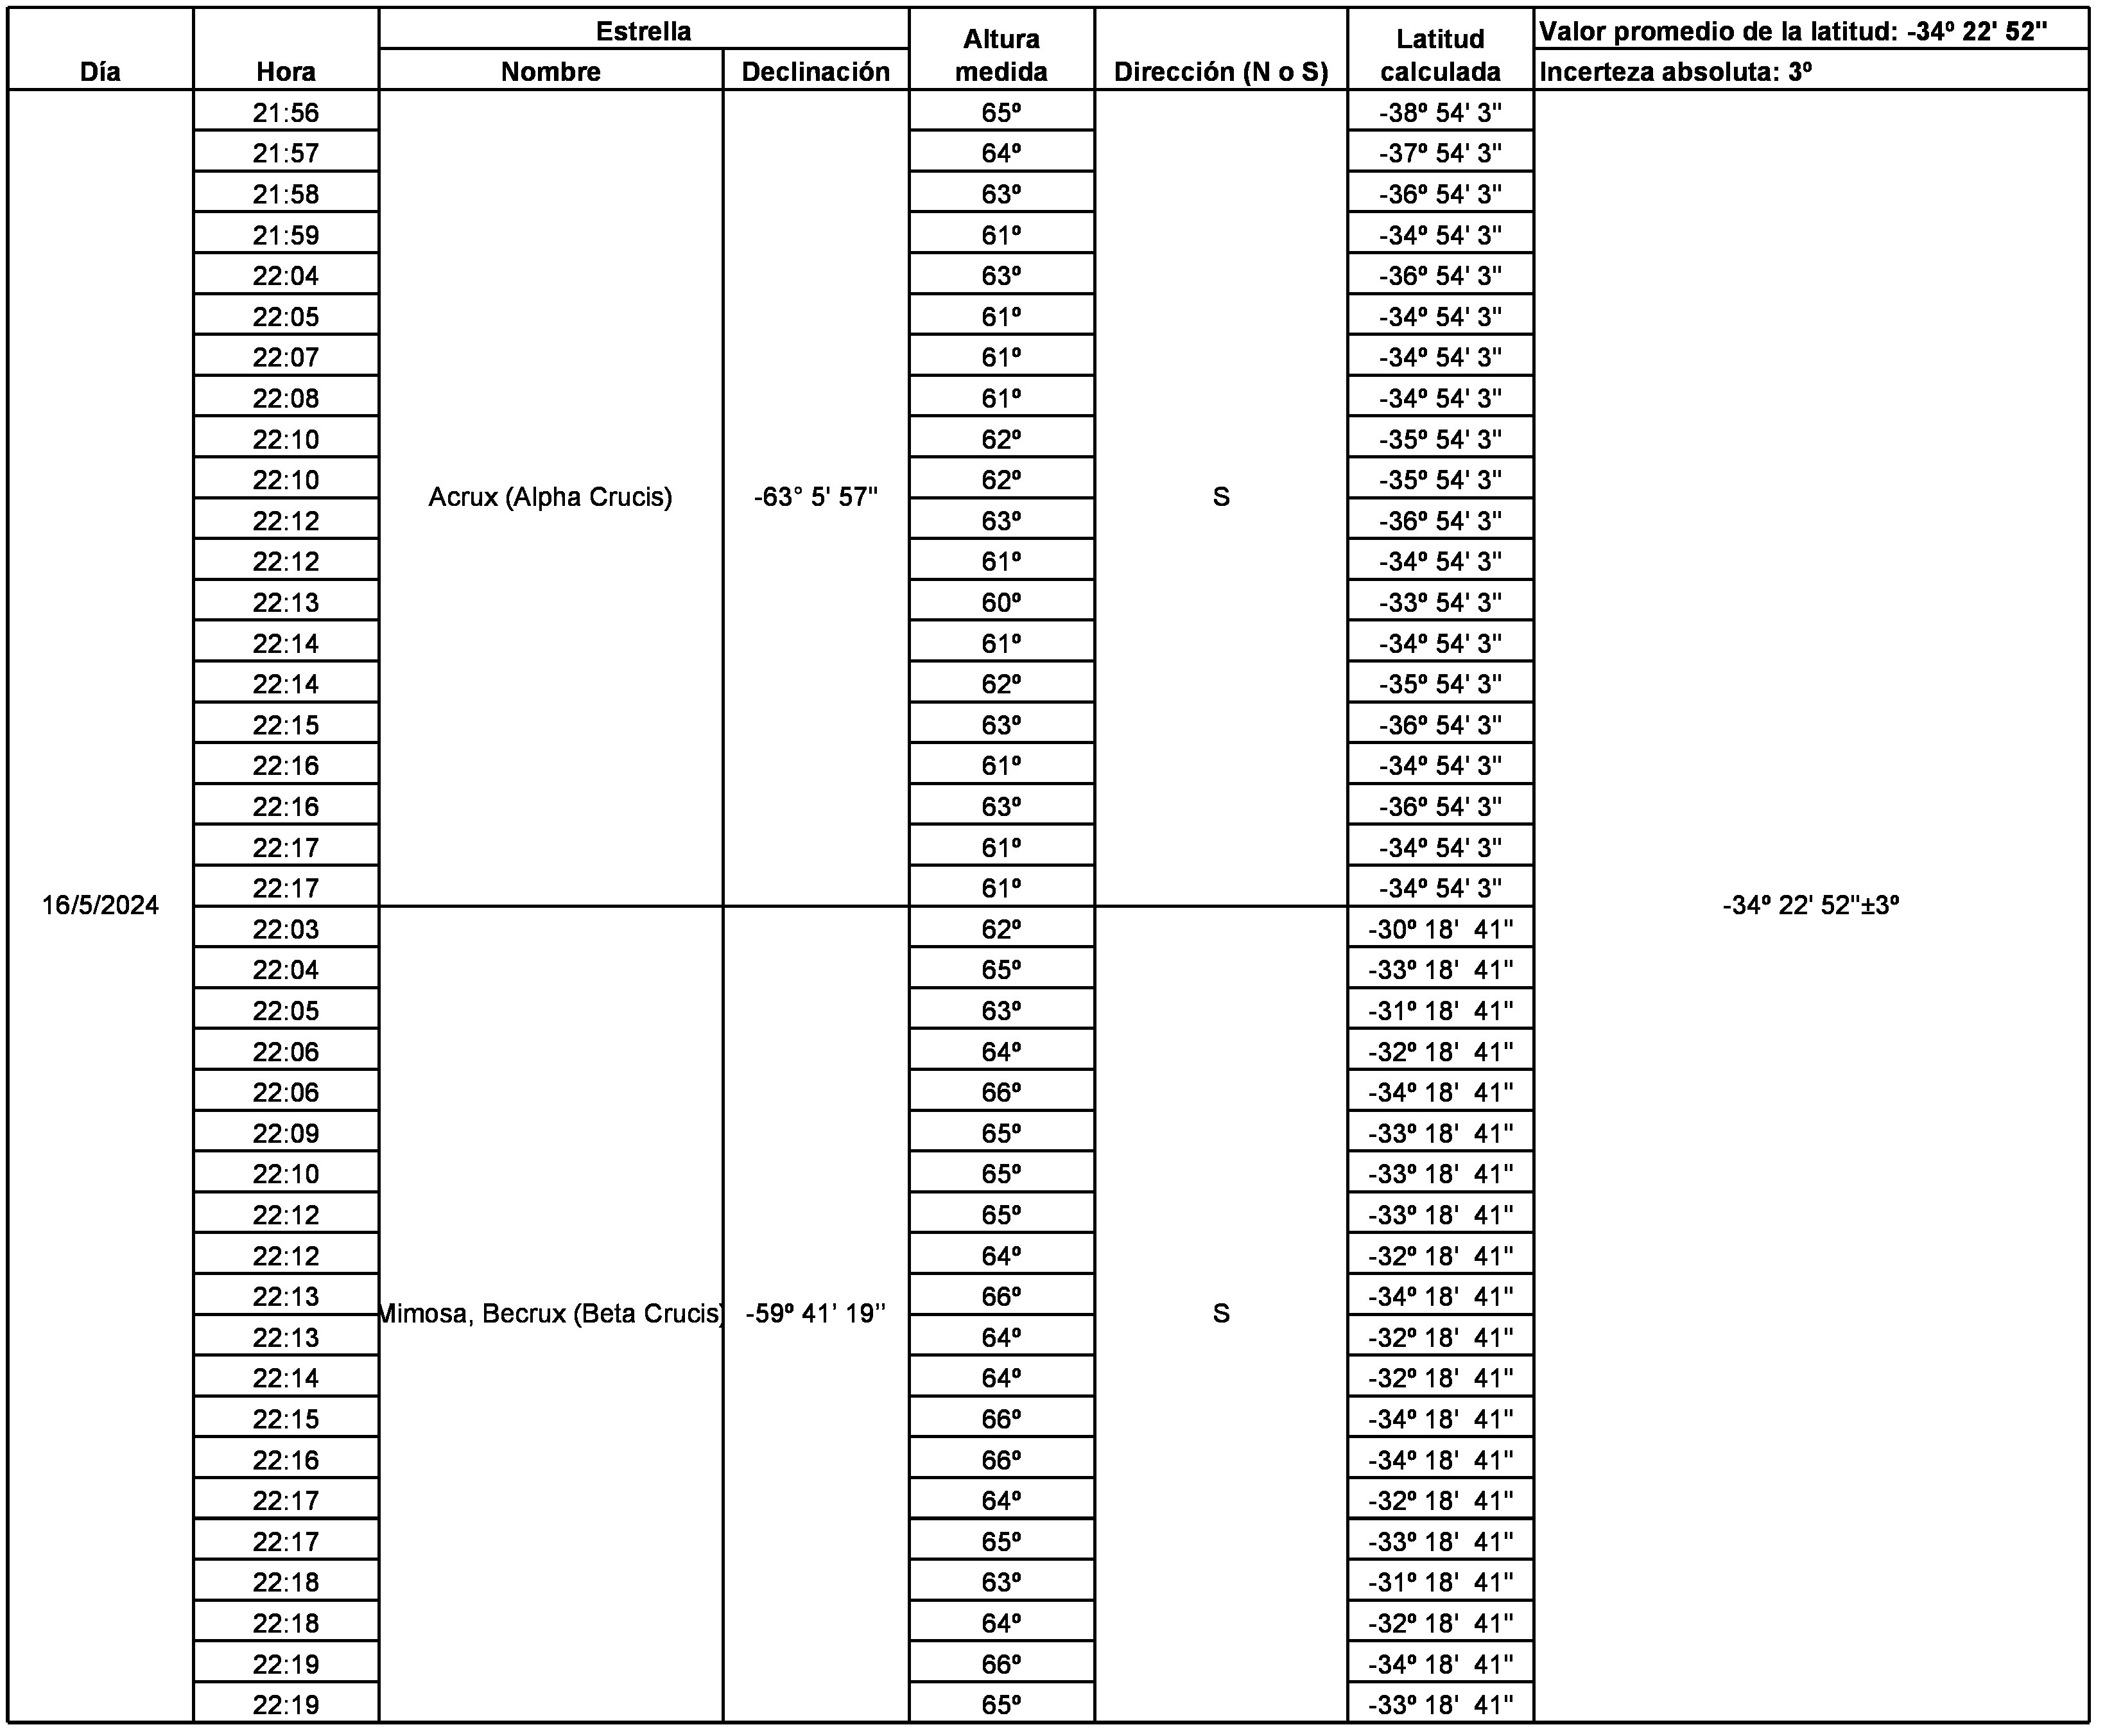
\includegraphics[width=15cm]{images/tabla-TP-1-Ian_Chen_y_Lola_Cavalieri .jpg}
    \caption{Tabla de mediciones}
    \label{fig:tabla-mediciones}
\end{figure}

Para completar la Tabla se tomaron mediciones de dos estrellas de la Cruz del Sur: Acrux y Becrux, cuyas declinaciones son $-\ang{63} \,5\text{'}\, 57\text{''}$ y $-\ang{59} \, 41\text{'}\, 19\text{''}$ respectivamente \cite{buenosairesPlanetarioGalileo}. Se puede observar que las latitudes calculadas para Acrux muestran un rango de $-\ang{38} \,54\text{'}\, 3\text{''}$ a $-\ang{33} \,54\text{'}\, 3\text{''}$ mientras que las latitudes calculadas para Becrux muestran un rango de $-\ang{34} \,18\text{'}\, 41\text{''}$ a $-\ang{30} \,18\text{'}\, 41\text{''}$. En conjunto el valor promedio de las latitudes calculadas para ambas estrellas es $-\ang{34} \,22\text{'}\, 52\text{''}$. La variabilidad en las mediciones es significativa, con un rango de $\ang{5}$ para Acrux y $\ang{4}$ para Becrux. Esta variabilidad puede deberse a varios factores como errores de observación, condiciones atmosféricas cambiantes, y la precisión del equipo de medición (un cuadrante en este caso).

\subsection{Histograma}
%Análisis de histograma
\begin{figure}[H]
    \centering
    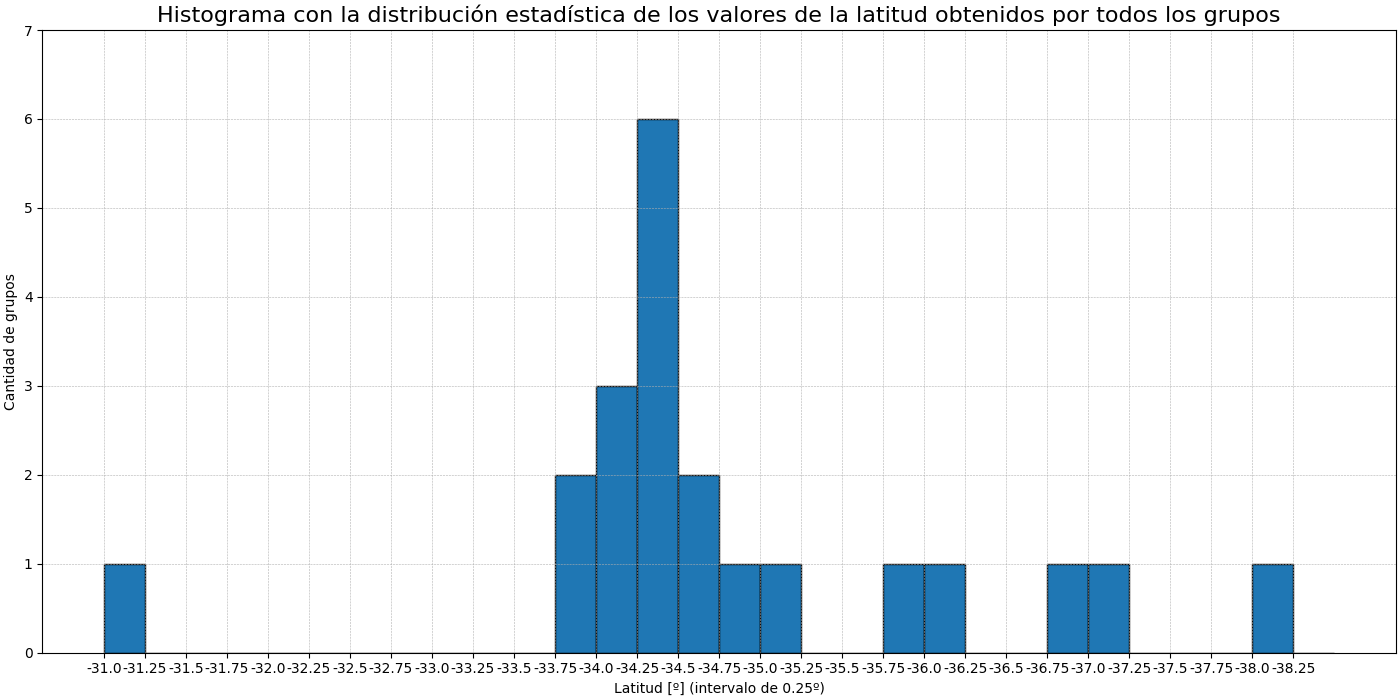
\includegraphics[width=15cm]{images/histograma.png}
    \caption{Histograma con la distribución estadística de los valores de la latitud obtenidos por todos los grupos del curso.}
    \label{fig:histograma}
\end{figure}

Podemos ver en el histograma de la Figura 3 que varios grupos obtuvieron valores entre $-\ang{34}$ y $-\ang{34.75}$. A primera vista ya vemos que 6 grupos obtuvieron valores de $-\ang{34.25}$ y $-\ang{34.5}$ mientras que pocos grupos (6 para ser exactos) obtuvieron valores más alejados. Los valores más extremos, entre $-\ang{31}$ y $-\ang{31.25}$ y entre $-\ang{38}$ y $-\ang{38.25}$, se pueden descartar ya que al ser un proceso experimental se esperan fallas y resultados con variaciones, por lo que se toma un promedio de los datos. De todas formas la concordancia de la gran mayoría de los grupos en el valor promedio de la latitud demuestra que estos utilizaron los mismos recursos y el mismo método en sus mediciones y cálculos. 

\subsection{Gráfico}
% Análisis de Gráfico
\begin{figure}[H]
    \centering
    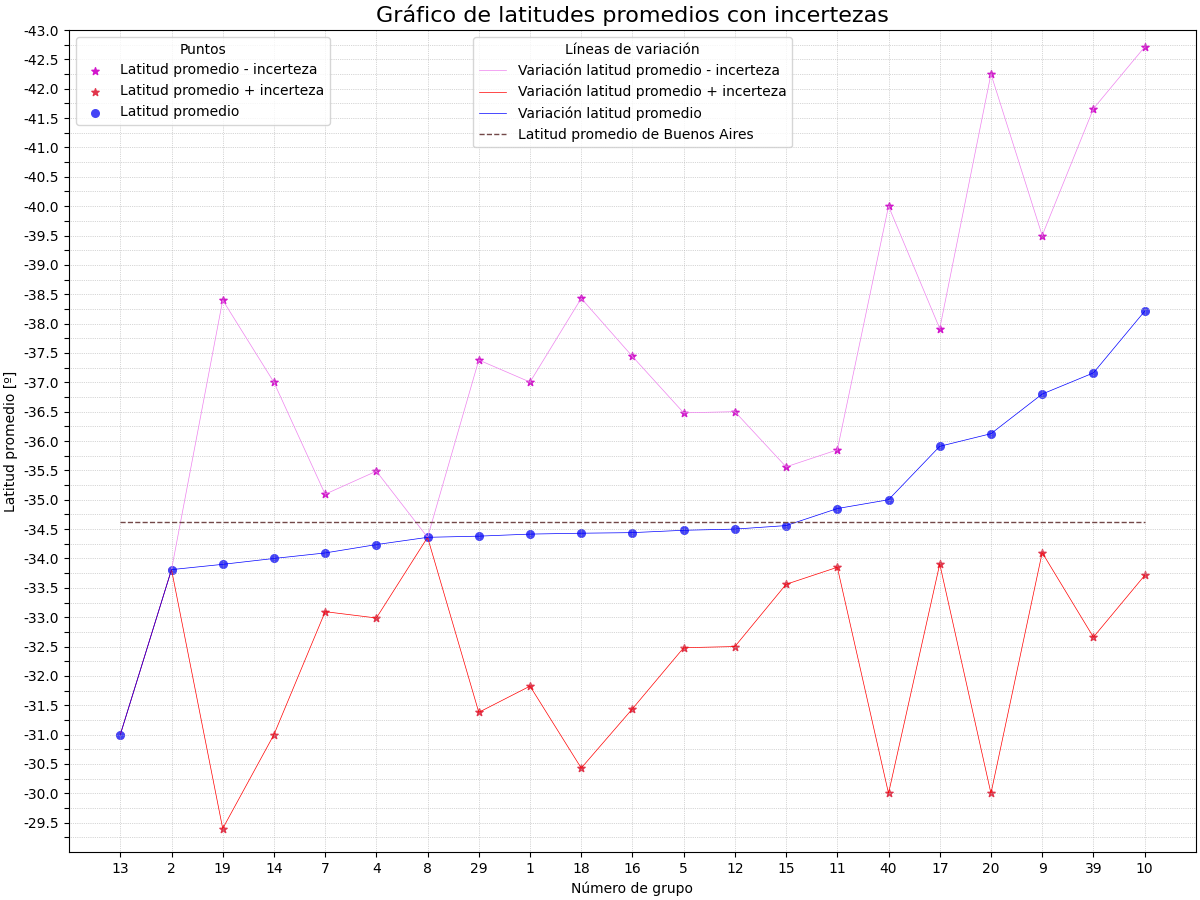
\includegraphics[width=15cm]{images/gráfico_análisis.png}
    \caption{Gráfico de latitudes promedios con incertezas de cada grupo}
    \label{fig:grafico}
\end{figure}

Para un mejor análisis se confeccionó un gráfico utilizando valores de latitud promedios obtenidos y las incertezas asignadas por grupo como muestra en la Figura \ref{fig:grafico}.

En el gráfico se puede apreciar cómo la mayoría de los valores promedios de latitud obtenidos (en azul) respetan un cierto margen, con variaciones no mayores a $\ang{3}$ en los valores útiles para el estudio. Se observa que los grupos 13 y 10 tuvieron los valores más extremos. Pero como se mencionó anteriormente en el análisis del histograma, los valores extremos pueden descartarse en el análisis, ya que son menos representativos del conjunto de datos.

También podemos observar varias líneas que unen los puntos obtenidos de cada grupo. Estos sirven de ayuda visual y para mejor comprensión del análisis. En el caso de la línea azul que une los valores promedios de latitud obtenidos, podemos notar que la pendiente \textbf{no} es pronunciada y que los valores medios son cercanos a la línea negra que representa la latitud de Buenos Aires. 

Adicionalmente, se puede observar que cada grupo eligió un valor diferente de incerteza, lo que resultó en una curva más pronunciada y una amplia variación en los valores promedio de latitud cuando se tenía en cuenta la incerteza asignada. Esto demuestra que la estimación de ésta tiene un impacto significativo en los resultados obtenidos. Se observa una gran variación de $\ang{13.25}$ entre el valor máximo de $-\ang{42.75}$ (obtenido por el grupo 10) y el valor mínimo de $-\ang{29.5}$ (obtenido por el grupo 19). Las líneas que unen los promedios $\pm$ incerteza no siguen ningún patrón específico, ya que cada grupo asignó un valor distinto. Esta información es relevante porque indica que ningún grupo compartió información de su trabajo, lo que llevó a la asignación de diferentes valores de incerteza (dado que era de libre elección), a diferencia del valor promedio de latitud, el cual se calculaba mediante el mismo procedimiento. Aunque algunos grupos obtuvieron valores cercanos a la latitud de Buenos Aires, la variación en la estimación de las incertezas desorganizó los resultados.

%--------------------------
\section{Conclusiones}
Los objetivos de este trabajo práctico fueron tres principalmente: la utilización de un instrumento astronómico (cuadrante), la realización de un experimento científico (de lo práctico a la redacción de informe), y la relación entre los conceptos astronómicos de altura, declinación, la latitud, y el meridiano del lugar. 

Luego del análisis detallado en el informe se pudo llegar a la conclusión que la latitud aproximada del lugar de observación es de -34º22’52’’ (en nuestro caso), la cual es cercana a la latitud estimada de Buenos Aires: $-\ang{34} \, 36\text{'} \, 47.3\text{''}$ {\cite{geodatosCoordenadasGeogrxE1ficas}}. 
Esto valida la efectividad de la utilización de métodos tradicionales y antiguas para mediciones aproximadas. Este método de medición con un cuadrante, el cual es instrumento sencillo y de fácil acceso, puede ser útil en áreas remotas donde no hay tecnología avanzada como telescopios o GPS. 

El hecho de que la latitud hallada pueda ser aproximada a la actual indica que se aplicaron de manera correcta no sólo la parte instrumental sino que también la teórica al poder aplicar conocimientos astronómicos y relacionarlas matemáticamente para formular ecuaciones, y finalmente hallar una latitud aproximada. 

En conclusión, fue un trabajo que abordó distintos temas y aspectos del trabajo científico, el cual ayudó a profundizar temas básicos de astronomía y la utilización práctica por fuera de lo teórico para aplicarlo en la vida cotidiana.
\hfill

%---------------------------
\singlespacing
\section{Apéndice}
\subsection{Ecuaciones de latitud según ubicación de la estrella}

\selectlanguage{english}
%----------SUR-----------
\begin{figure}[H]
    \centering
    \begin{subfigure}{0.3\textwidth}
        \begin{tikzpicture}[scale=0.8]
            % Circunferencia
            \draw[black, thick] (0,0) circle (2);
            
            % Rectas / Líneas
            \draw[black, very thin] (-2, 0) -- (2, 0) node[anchor=west]{H};
            \draw[black, very thin] (-1.65, -1.19) -- (1.65, 1.19) node[anchor=south west]{PSC};
            \draw[black, very thin]  (1.19, -1.65) -- (-1.19, 1.65)  node[anchor=south east]{EC};
            % Línea roja
            \draw[red!70, dashed] (0,0) -- (-1.76, 0.93);
        
            % Arcos
            % Declinación
            \draw[cyan!40, very thick, ->] (-1.17, 1.74) arc (124:150:2.1) node[midway, left]{$\delta$};
            % Altura h
            \draw[blue!40, very thick, ->] (-2.1, 0) arc (180:158:2.1) node[midway, left]{$h$};
            \draw[black, thick, ->] (1, 0) arc (0:34:1) node[midway, right]{$\varphi$};
            
            % % Cuadrados
            \draw[black, very thin, rotate around={34:(0,0)}] (0,0) rectangle (0.3, 0.35);
        
            % % Puntos
            \filldraw[fill=black!50, draw=black!50] (0,0) circle (0.1);
            % Estrella a 152º
            \filldraw[fill=yellow, draw=yellow] (-1.76, 0.93) circle (0.1); 
        \end{tikzpicture}
        \caption{$\varphi = h + \delta - \ang{90}$}
    \end{subfigure}
    \hspace{0.1cm}
    \hfill
    \begin{subfigure}{0.3\textwidth}
        \begin{tikzpicture}[scale=0.8]
            % Circunferencia
            \draw[black, thick] (0,0) circle (2);
            
            % Rectas / Líneas
            \draw[black, very thin] (-2, 0) -- (2, 0) node[anchor=west]{H};
            \draw[black, very thin] (-1.65, -1.19) -- (1.65, 1.19) node[anchor=south west]{PSC};
            \draw[black, very thin]  (1.19, -1.65) -- (-1.19, 1.65)  node[anchor=south east]{EC};
            % Línea roja
            \draw[red!70, dashed] (0,0) -- (0, 2);
        
            % Arcos
            % Declinación
            \draw[cyan!40, very thick, ->] (-1.17, 1.74) arc (124:94:2.1) node[midway, above]{$\delta$};
            % Altura h
            \draw[blue!40, very thick, ->] (2.1, 0) arc (0:86:2.1) node[midway, above]{$h$};
            \draw[black, thick, ->] (1, 0) arc (0:34:1) node[midway, right]{$\varphi$};
            
            % % Cuadrados
            \draw[black, very thin, rotate around={34:(0,0)}] (0,0) rectangle (0.3, 0.35);
        
            % % Puntos
            \filldraw[fill=black!50, draw=black!50] (0,0) circle (0.1);
            % Estrella a 90º
            \filldraw[fill=yellow, draw=yellow] (0, 2) circle (0.1); 
        \end{tikzpicture}
        \caption{$\varphi = \ang{90} + \delta - h$}
    \end{subfigure}
    % \hspace{0.05cm}
    \hfill
    \begin{subfigure}{0.3\textwidth}
        \begin{tikzpicture}[scale=0.8]
            % Circunferencia
            \draw[black, thick] (0,0) circle (2);
            
            % Rectas / Líneas
            \draw[black, very thin] (-2, 0) -- (2, 0) node[anchor=west]{H};
            \draw[black, very thin] (-1.65, -1.19) -- (1.65, 1.19) node[anchor=south west]{PSC};
            \draw[black, very thin]  (1.19, -1.65) -- (-1.19, 1.65)  node[anchor=south east]{EC};
            % Línea roja
            \draw[red!70, dashed] (0,0) -- (1.91, 0.58);
        
            % Arcos
            % Declinación
            \draw[cyan!40, very thick, ->] (1.17, -1.74) arc (-56:13:2.1) node[midway, below]{$\delta$};
            % Altura h
            \draw[blue!40, very thick, ->] (1.9, 0) arc (0:13:1.9) node[midway, left]{$h$};
            \draw[black, thick, ->] (1, 0) arc (0:34:1) node[midway, right]{$\varphi$};
            
            % % Cuadrados
            \draw[black, very thin, rotate around={34:(0,0)}] (0,0) rectangle (0.3, 0.35);
        
            % % Puntos
            \filldraw[fill=black!50, draw=black!50] (0,0) circle (0.1);
            % Estrella a 17º
            \filldraw[fill=yellow, draw=yellow] (1.91, 0.58) circle (0.1); 
        \end{tikzpicture}
        \caption{$\varphi = \delta - h - \ang{90}$}
    \end{subfigure}  
    \caption{Ecuaciones de latitud en hemisferio sur}
    \label{fig:lat-hemisferio-sur}
\end{figure}


%----------NORTE-------------
\begin{figure}[H]
    \centering
    \begin{subfigure}{0.3\textwidth}
        \begin{tikzpicture}[scale=0.8]
            % Circunferencia
            \draw[black, thick] (0,0) circle (2);
            
            % Rectas / Líneas
            \draw[black, very thin] (-2, 0) -- (2, 0) node[anchor=west]{H};
            \draw[black, very thin] (-1.65, -1.19) -- (1.65, 1.19) node[anchor=south west]{PNC};
            \draw[black, very thin]  (1.19, -1.65) -- (-1.19, 1.65)  node[anchor=south east]{EC};
            % Línea roja
            \draw[red!70, dashed] (0,0) -- (-1.76, 0.93);
        
            % Arcos
            % Declinación
            \draw[cyan!40, very thick, ->] (-1.17, 1.74) arc (124:150:2.1) node[midway, left]{$\delta$};
            % Altura h
            \draw[blue!40, very thick, ->] (-2.1, 0) arc (180:158:2.1) node[midway, left]{$h$};
            \draw[black, thick, ->] (1, 0) arc (0:34:1) node[midway, right]{$\varphi$};
            
            % % Cuadrados
            \draw[black, very thin, rotate around={34:(0,0)}] (0,0) rectangle (0.3, 0.35);
        
            % % Puntos
            \filldraw[fill=black!50, draw=black!50] (0,0) circle (0.1);
            % Estrella a 152º
            \filldraw[fill=yellow, draw=yellow] (-1.76, 0.93) circle (0.1); 
        \end{tikzpicture}
        \caption{$\varphi = \ang{90} + \delta - h$}
    \end{subfigure}
    \hspace{0.1cm}
    \hfill
    \begin{subfigure}{0.3\textwidth}
        \begin{tikzpicture}[scale=0.8]
            % Circunferencia
            \draw[black, thick] (0,0) circle (2);
            
            % Rectas / Líneas
            \draw[black, very thin] (-2, 0) -- (2, 0) node[anchor=west]{H};
            \draw[black, very thin] (-1.65, -1.19) -- (1.65, 1.19) node[anchor=south west]{PNC};
            \draw[black, very thin]  (1.19, -1.65) -- (-1.19, 1.65)  node[anchor=south east]{EC};
            % Línea roja
            \draw[red!70, dashed] (0,0) -- (0, 2);
        
            % Arcos
            % Declinación
            \draw[cyan!40, very thick, ->] (-1.17, 1.74) arc (124:94:2.1) node[midway, above]{$\delta$};
            % Altura h
            \draw[blue!40, very thick, ->] (2.1, 0) arc (0:86:2.1) node[midway, above]{$h$};
            \draw[black, thick, ->] (1, 0) arc (0:34:1) node[midway, right]{$\varphi$};
            
            % % Cuadrados
            \draw[black, very thin, rotate around={34:(0,0)}] (0,0) rectangle (0.3, 0.35);
        
            % % Puntos
            \filldraw[fill=black!50, draw=black!50] (0,0) circle (0.1);
            % Estrella a 90º
            \filldraw[fill=yellow, draw=yellow] (0, 2) circle (0.1); 
        \end{tikzpicture}
        \caption{$\varphi = h + \delta -\ang{90}$}
    \end{subfigure}
    % \hspace{0.05cm}
    \hfill
    \begin{subfigure}{0.3\textwidth}
        \begin{tikzpicture}[scale=0.8]
            % Circunferencia
            \draw[black, thick] (0,0) circle (2);
            
            % Rectas / Líneas
            \draw[black, very thin] (-2, 0) -- (2, 0) node[anchor=west]{H};
            \draw[black, very thin] (-1.65, -1.19) -- (1.65, 1.19) node[anchor=south west]{PNC};
            \draw[black, very thin]  (1.19, -1.65) -- (-1.19, 1.65)  node[anchor=south east]{EC};
            % Línea roja
            \draw[red!70, dashed] (0,0) -- (1.91, 0.58);
        
            % Arcos
            % Declinación
            \draw[cyan!40, very thick, ->] (1.17, -1.74) arc (-56:13:2.1) node[midway, below]{$\delta$};
            % Altura h
            \draw[blue!40, very thick, ->] (1.9, 0) arc (0:13:1.9) node[midway, left]{$h$};
            \draw[black, thick, ->] (1, 0) arc (0:34:1) node[midway, right]{$\varphi$};
            
            % % Cuadrados
            \draw[black, very thin, rotate around={34:(0,0)}] (0,0) rectangle (0.3, 0.35);
        
            % % Puntos
            \filldraw[fill=black!50, draw=black!50] (0,0) circle (0.1);
            % Estrella a 17º
            \filldraw[fill=yellow, draw=yellow] (1.91, 0.58) circle (0.1); 
        \end{tikzpicture}
        \caption{$\varphi = \ang{90} + h - \delta$}
    \end{subfigure}  
    \caption{Ecuaciones de latitud en hemisferio norte}
    \label{fig:lat-hemisferio-norte}
\end{figure}
\selectlanguage{spanish}

\subsection{Deducción de fórmula de latitud utilizada}
Deducción de la ecuación correspondiente para hallar latitud $\varphi$ en este caso Figura 5b:
\begin{align*}
    |h|-|\varphi| &= \ang{90}-|\delta| \\
    |\varphi| &= -\ang{90}+|h|+|\delta| \\
    -\varphi &= -\ang{90} + h - \delta \\
    \varphi &= \ang{90} + \delta - h
\end{align*}
Para hallar valor de latitud para cada valor de altura se utilizó un script en Python que se encuentra en el \href{https://github.com/ianchu0317/TP1-astronomia-cuadrantes/tree/main}{repositorio de GitHub}.

\subsection{Incerteza de latitud}
Incerteza de altura $\varepsilon h = \ang{3}$\\[6pt]
Incerteza de latitud $\varepsilon \varphi = \ang{3}$\\[6pt]
Incerteza de promedio de latitud 
\begin{align*}
    \displaystyle \varepsilon \overline{\varphi} &= \frac{\varepsilon \varphi + \dots + \varepsilon \varphi}{n}\,\, : n=40\\[6pt]
    &= \frac{\ang{3} + \dots + \ang{3}}{40}\\[6pt]
    &= \frac{\ang{3} \cdot 40}{40} = \ang{3}
\end{align*}



\vspace{0.5cm}
%----------------------------
\hline
\bibliographystyle{apacite}
\bibliography{bibliografia}
\begin{itemize}
    \item Repositorio del Trabajo Práctico en GitHub: \url{https://github.com/ianchu0317/TP1-astronomia-cuadrantes/} 
\end{itemize}

\end{document}